% =============================================================================
% PNV3425 - Projeto de Sistemas Oceânicos - Trabalho Final - Grupo 02
% Versão: CONDIÇÃO DE 10% DE LASTRO
% Compilar com XeLaTeX ou Tectonic, na pasta relatorio/:
%     tectonic relatorio_condicao_10pct_lastro.tex
% As tabelas de resultados (tabelas/*.tex) são geradas por
%     python codigo/analises_condicao_10pct_lastro.py
% =============================================================================
\documentclass[11pt,a4paper]{article}

\usepackage{fontspec}
\usepackage[brazil]{babel}
\usepackage[a4paper,margin=2.3cm]{geometry}
\usepackage{amsmath,amssymb}
\usepackage{icomma}
\usepackage{graphicx}
\usepackage{booktabs}
\usepackage{array}
\usepackage{multirow}
\usepackage{longtable}
\usepackage{float}
\usepackage{caption}
\usepackage{xcolor}
\usepackage{enumitem}
\usepackage[hidelinks]{hyperref}

\graphicspath{{../resultados_lastro10/}{../resultados_lastro10/complementar/}{../../caso_base/resultados/complementar/}}
\captionsetup{font=small,labelfont=bf}
\setlist{itemsep=2pt,topsep=4pt}
\renewcommand{\arraystretch}{1.12}

\newcommand{\integrantes}{Felipe Perpétuo Simões -- 11263255\\[2pt]
  Gustavo Guilherme Silva -- 11820555\\[2pt]
  João Marcos Magalhães Moura -- 12554693}
\newcommand{\phial}{\varphi_{\mathrm{al}}}
\newcommand{\Hz}{H_{1/3,z}}
% \input expansível (primitivo): permite inserir linhas de tabela geradas pelo Python
\makeatletter\newcommand{\linhas}[1]{\@@input #1 }\makeatother

\begin{document}

% =============================================================================
\begin{titlepage}
\centering
{\large ESCOLA POLITÉCNICA DA UNIVERSIDADE DE SÃO PAULO\par}
{\large Departamento de Engenharia Naval e Oceânica\par}
\vspace{2.5cm}
{\Large PNV3425 -- Projeto de Sistemas Oceânicos\par}
\vspace{1.2cm}
{\LARGE\bfseries Projeto Paramétrico de uma Plataforma\\[4pt] Semissubmersível de Produção\par}
\vspace{0.8cm}
{\Large Bloco KZ-2026-B -- Bacia do Baixo Congo (Angola)\par}
\vspace{0.6cm}
{\Large\bfseries Condição de 10\% de lastro\par}
\vspace{0.2cm}
{\large $V_{lastro} \ge 0{,}10\,V_{pontoons}$\par}
\vspace{2.0cm}
{\large Grupo 02\par}
\vspace{0.4cm}
{\normalsize \integrantes\par}
\vfill
{\large São Paulo, novembro de 2026\par}
\end{titlepage}

% =============================================================================
\begin{abstract}
Esta é a versão \emph{Condição de 10\% de lastro} do projeto paramétrico da semissubmersível de
produção do bloco KZ-2026-B, em 1.450~m de lâmina d'água na bacia do Baixo Congo. O modelo, os
dados e os objetivos são os mesmos do caso-base (mínimo peso estrutural do casco e mínimo $\Hz$
de \emph{heave}); a única diferença é uma restrição adicional obrigatória, $V_{lastro} \ge
0{,}10\,V_{pontoons}$, que reserva capacidade de lastro para ajuste de calado e de trim e para
compensar crescimento de peso. A otimização (20.000 amostras de hipercubo latino, soma
ponderada e $\varepsilon$-restrito com SLSQP e filtro de não dominância) produz uma fronteira de
Pareto de 23 pontos, entre 11.892~t ($\Hz = 2{,}36$~m) e 23.634~t ($\Hz = 1{,}04$~m). A solução
escolhida, no joelho da fronteira, tem $L_p = 107{,}5$~m, $T = 25{,}9$~m, casco de 16.026~t,
3.611~t de lastro, $\Hz = 1{,}55$~m, $T_n = 21{,}7$~s e $A/B = 1{,}303$. Em relação ao caso-base, o
casco fica 6,9\% mais pesado, o KG cai 4,44~m e o \emph{heave} praticamente não muda; o
deslocamento específico (285~t por mil bopd) passa ao nível da Troll C, a semissubmersível mais
enxuta do pôster de 2011.
\end{abstract}

\tableofcontents
\newpage

% =============================================================================
\section{Introdução}

O caso-base do projeto segue a letra do enunciado, que exige apenas lastro positivo. Nele, a
solução escolhida tem só 11~t de lastro, uma margem numérica: casco, \emph{topside},
\emph{risers} e amarração consomem todo o deslocamento, e a plataforma não teria como ajustar
calado e trim nem compensar crescimento de peso ao longo da vida útil.

Esta versão repete o projeto inteiro com uma restrição adicional obrigatória:
\begin{equation}
V_{lastro} \ge 0{,}10\,V_{pontoons}, \qquad V_{pontoons} = 2 L_p b_p h_p ,
\end{equation}
isto é, pelo menos 10\% do volume interno dos \emph{pontoons} deve estar ocupado por lastro na
condição de projeto. Os dados do campo, o modelo paramétrico, a validação, os limites das
variáveis, os objetivos e as demais restrições são idênticos aos do caso-base, cujo relatório
detalha as equações. Este relatório apresenta os resultados da otimização com a nova restrição,
a solução escolhida e a comparação com o caso-base e com a frota real.

% =============================================================================
\section{Dados do campo e de projeto}

\begin{table}[H]
\centering
\caption{Características do bloco KZ-2026-B e mar de projeto.}\label{tab:campo}
\begin{tabular}{ll}
\toprule
Item & Valor \\
\midrule
Lâmina d'água · distância à costa & 1.450 m · 190 km \\
Óleo original · grau API & 2,2 bilhões de bbl · 31 \\
Fator de recuperação & 30\% (660 milhões de bbl) \\
Gás recuperável & 30 bilhões de m$^3$ \\
Pico de produção de óleo & 158.894,48 bpd (anos 5 a 7) \\
Mar de 100 anos & $H_s = 5{,}6$ m · $T_p = 15{,}2$ s \\
Vento de 100 anos · corrente na superfície & 24 m/s · 0,95 m/s \\
\bottomrule
\end{tabular}
\end{table}

\begin{table}[H]
\centering
\caption{Dados fixos do projeto (iguais aos do caso-base).}\label{tab:fixos}
\small
\begin{tabular}{llr}
\toprule
Dado & Símbolo & Valor \\
\midrule
Produção de pico (só óleo) & BOE & 158.894,48 boe/dia \\
Área mínima de convés & $42{,}246Q + 4850{,}1$ & 11.563 m$^2$ ($L_p \ge 107{,}53$ m) \\
Planta de produção & 0,083 t/boe & 13.188 t \\
\emph{Topside} (planta + 35\% convés + 35\% carga) & $W_{top}$ & 22.420 t \\
Peso específico estrutural & $\gamma_e$ & 0,270 t/m$^3$ \\
Altura do \emph{deck box} · dos módulos & $h_d$ · $h_m$ & 8 · 12 m \\
Vento de tempestade / operação & $V$ & 51,5 / 36 m/s \\
Amortecimento em \emph{heave} · JONSWAP & $\xi$ · $\gamma$ & 0,05 · 3,3 \\
\textbf{Lastro mínimo obrigatório} & $V_{lastro}/V_{pontoons}$ & \textbf{0,10} \\
\bottomrule
\end{tabular}
\end{table}

\begin{figure}[H]
\centering
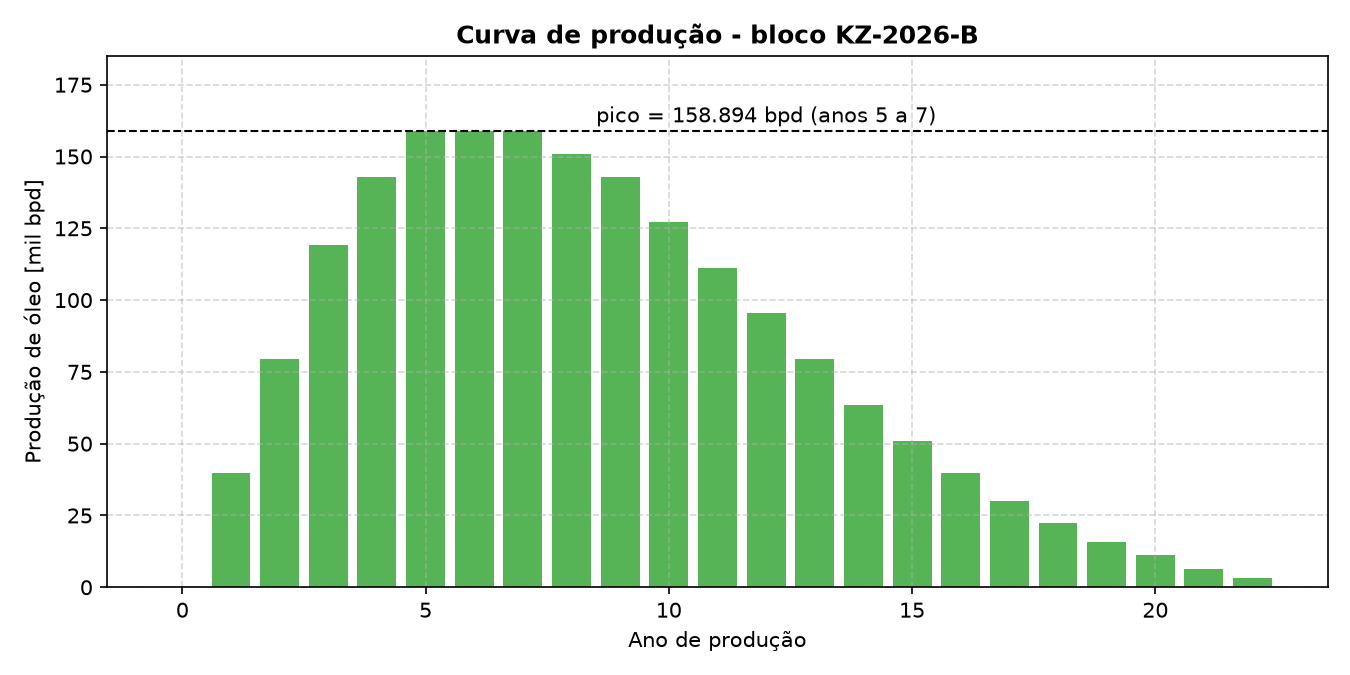
\includegraphics[width=0.72\textwidth]{06_curva_producao.png}
\caption{Curva de produção de óleo do campo KZ-2026-B.}\label{fig:producao}
\end{figure}

% =============================================================================
\section{Modelo paramétrico e restrições}

O modelo é o mesmo do caso-base. Para cada conjunto $x = (L_p, b_p, h_p, b_c, h_c, T)$ ele
calcula, em sequência:
\begin{enumerate}
\item hidrostática: $\nabla = 2L_pb_ph_p + 4b_c^2(T-h_p)$, $\Delta = \rho\nabla$, KB, BM e KM
(Exercício 7);
\item pesos e centros: casco $\gamma_e(2L_pb_ph_p + 4b_c^2h_c)$, \emph{topside}, \emph{risers}
(4\% $\Delta$), amarração (3\% $\Delta$) e lastro $= \Delta - \sum W$, posicionado no nível real
de enchimento dos \emph{pontoons}; KG e GM (Exercício 8);
\item área de convés $L_p^2$ e \emph{air gap} $a = h_p + h_c - T$ (Exercício 8);
\item curva GZ de 0 a 50$^\circ$ por projeções 2D, a volume constante, nos dois planos, e
ângulo de alagamento $\phial$ (Exercício 9);
\item momento de vento com 4 colunas sem sombra, \emph{deck box}, módulos e face inferior do
convés, braço até o $z_{CLR}$ de cada plano, e critério de áreas
$A = \int_0^{\phial} GZ\,d\varphi \ge 1{,}3\int_0^{\phial} HA\,d\varphi$ (Exercício 9);
\item forças de \emph{heave} (Froude-Krylov e massa adicional, com o fator
$\cos(\omega^2 d_p/2g)$), $A_{33}$ com $l_d = L_p - 2b_c$, $T_n$ e RAO (Exercício 10);
\item espectro de resposta $S_z = RAO^2 S_\zeta$ no JONSWAP de 100 anos e
$\Hz = 4\sqrt{m_{0z}}$ (Exercício 10);
\item \emph{air gap} mínimo $a_{\text{mín}} = 1{,}86H_s/2 + 1{,}86\Hz/2$.
\end{enumerate}
O lastro entra no KG com centro em $n/2$, sendo $n = V_{lastro}/(2L_pb_p)$ o nível de
enchimento; é por isso que exigir lastro baixa o KG da plataforma.

\begin{table}[H]
\centering
\caption{Restrições do problema. A última linha é a restrição adicional desta versão.}\label{tab:restricoes}
\begin{tabular}{ll}
\toprule
Restrição & Expressão \\
\midrule
Área mínima de convés & $L_p^2 \ge 11.562{,}8$ m$^2$ \\
Estabilidade inicial & $1~\text{m} \le GM_T \le 4~\text{m}$ \\
Período natural de \emph{heave} & $T_n > 20$ s \\
Lastro (enunciado) & $W_{lastro} > 0$ e $V_{lastro} \le 0{,}9\, V_{pontoons}$ \\
Colunas e \emph{pontoons} & $b_c \le b_p$ \\
Critério de áreas & $\min A/B \ge 1{,}3$ e $GZ > 0$, nos 4 casos \\
\emph{Air gap} & $a \ge a_{\text{mín}}$ \\
Consistência geométrica & $T - h_p \ge 1$ m \\
\midrule
\textbf{Lastro mínimo obrigatório} & $\mathbf{V_{lastro} \ge 0{,}10\, V_{pontoons}}$ \\
\bottomrule
\end{tabular}
\end{table}

O domínio das variáveis é o do caso-base: $107{,}5 \le L_p \le 150$~m,
$8 \le b_p, b_c \le 25$~m, $6 \le h_p \le 20$~m, $20 \le h_c \le 50$~m e $12 \le T \le 40$~m.

% =============================================================================
\section{Validação}

Como o modelo não muda, a validação é a mesma do caso-base: a plataforma dos Exercícios 7 a 10
($L_p = 100$~m, $b_p = h_p = b_c = 15$~m, $h_c = 45$~m, $T = 30$~m) já tem lastro de 15.748~t,
34\% do volume dos \emph{pontoons}, e atende à nova restrição.

\begin{table}[H]
\centering
\caption{Validação contra os resultados das aulas (plataforma dos Exercícios 7 a 10).}\label{tab:valaula}
\begin{tabular}{lrrr}
\toprule
Grandeza & Modelo & Aula & Erro \\
\midrule
KG [m] & 33,213 & 33,00 & +0,6\% \\
$\min A/B$ transversal & 2,310 & 2,33 & $-0{,}9$\% \\
$\min A/B$ longitudinal & 2,273 & 2,36 & $-3{,}7$\% \\
$T_n$ [s] & 20,703 & 20,70 & 0,0\% \\
$\Hz$ [m] & 2,984 & 2,98 & +0,1\% \\
$\eta_{max}$ [m] & 11,346 & 11,35 & 0,0\% \\
\bottomrule
\end{tabular}
\end{table}

Aplicado a três semissubmersíveis reais de 2 \emph{pontoons} e 4 colunas do pôster de
2011~\cite{poster} (Veslefrikk B, Njord A e P-20), o modelo reproduz o deslocamento com erro de
até 10\% (detalhes no relatório do caso-base).

% =============================================================================
\section{Variação sistemática e fronteira de Pareto}\label{sec:otimizacao}

O procedimento é o do caso-base: (1) 20.000 amostras por hipercubo latino (semente 2026);
(2) soma ponderada $F = w_1\Hz + w_2 W_{casco}/10.000$ com SLSQP para $w_1 = 0; 0{,}05; \ldots; 1$,
partindo das 5 melhores amostras e do ótimo do $w_1$ anterior; (3) método $\varepsilon$-restrito,
$\min W_{casco}$ com $\Hz \le \varepsilon$, em 12 níveis; (4) filtro de não dominância, com cada
ótimo reconfirmado pela curva GZ a cada $0{,}25^\circ$.

\begin{itemize}
\item \textbf{Hipercubo latino.} Das 20.000 amostras, 517 atendem às restrições estáticas, de
\emph{heave}, de \emph{air gap} e de lastro, e 209 (1,0\%) também ao critério de áreas; o vento
reprova sozinho 308 cascos. A nova restrição tira 30 cascos do conjunto pré-viável (547 no
caso-base).
\item \textbf{Soma ponderada.} Os 21 valores de $w_1$ terminam em pontos viáveis; 7 ficam
dominados, porque a fronteira continua não convexa.
\item \textbf{$\varepsilon$-restrito.} Os 12 níveis terminam em pontos viáveis com
\texttt{success = True}.
\item \textbf{Fronteira.} Das 242 soluções viáveis (209 + 21 + 12), 23 são não dominadas: 12 da
soma ponderada e 11 do $\varepsilon$-restrito (Figura~\ref{fig:pareto}; lista completa no
Apêndice~\ref{ap:fronteira}). A rodada completa levou 176~s em 8 núcleos.
\end{itemize}

\begin{figure}[H]
\centering
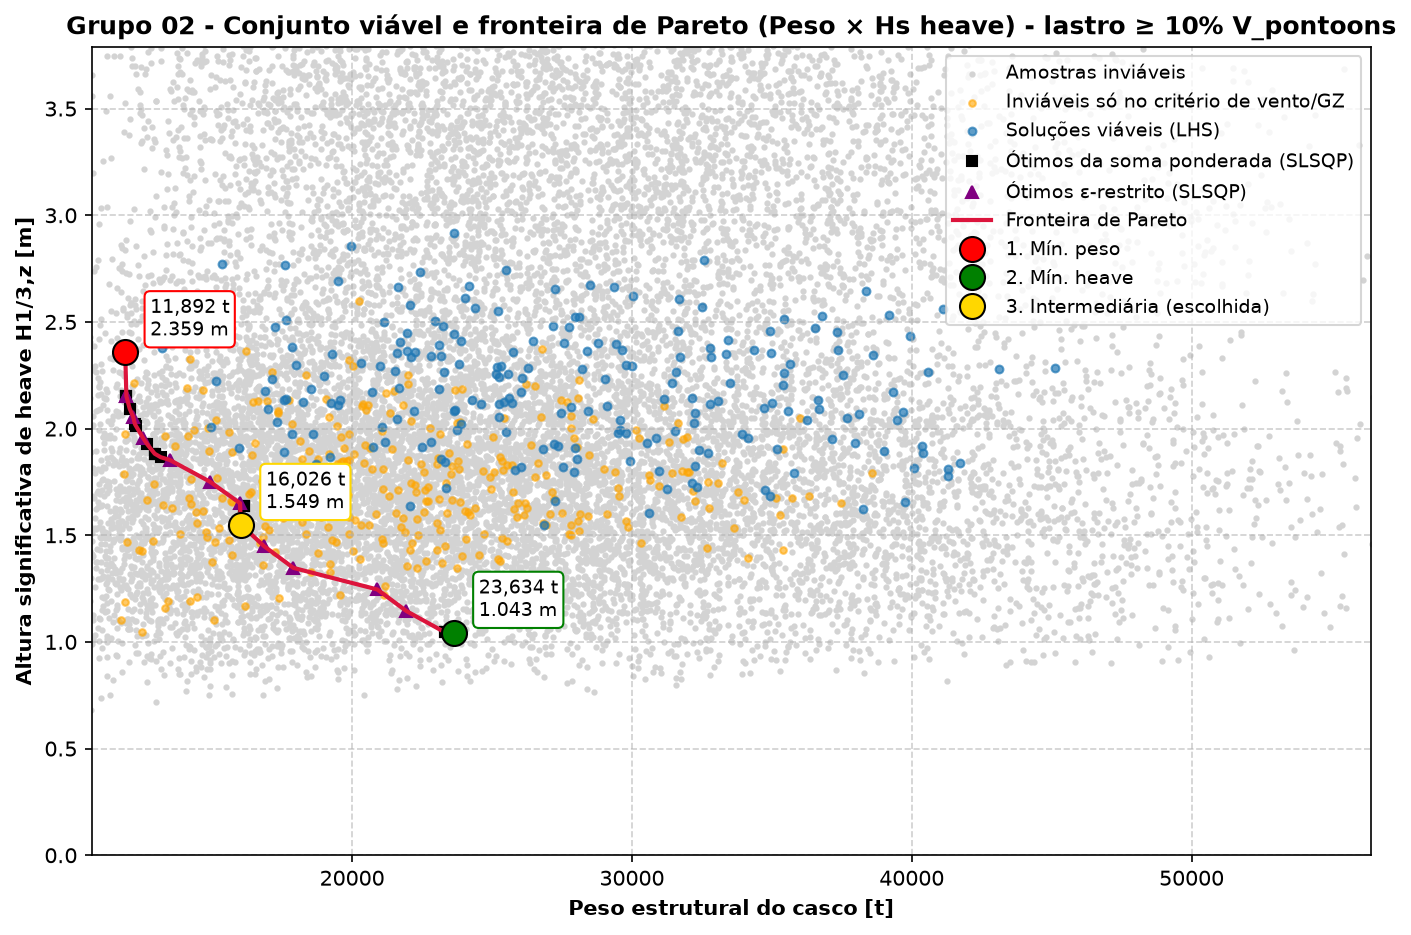
\includegraphics[width=0.92\textwidth]{01_pareto.png}
\caption{Conjunto viável e fronteira de Pareto na condição de 10\% de lastro.}\label{fig:pareto}
\end{figure}

\paragraph{Restrições ativas.} Como no caso-base, $GM_T = 4$~m e $A/B = 1{,}30$ estão ativos em
todos os pontos da fronteira (Tabela~\ref{tab:ativas}). A nova restrição de lastro está ativa em
16 dos 23 pontos: o otimizador põe exatamente o lastro mínimo, e só os cascos mais profundos
têm lastro acima dele. \emph{Air gap} e $T_n$ nunca são ativos.

\begin{table}[H]
\centering
\caption{Restrições ativas ao longo da fronteira de Pareto.}\label{tab:ativas}
\begin{tabular}{lr}
\toprule
Restrição ativa & Pontos \\
\midrule
$GM_T = 4$~m & 23 / 23 \\
$A/B = 1{,}30$ & 23 / 23 \\
$V_{lastro} = 0{,}10\,V_{pontoons}$ & 16 / 23 \\
$b_c = b_p$ & 7 / 23 \\
área de convés mínima & 6 / 23 \\
\emph{Air gap} e $T_n$ & 0 / 23 \\
\bottomrule
\end{tabular}

\end{table}

\paragraph{Famílias de projeto.} A Figura~\ref{fig:variaveis} mostra as mesmas duas famílias
do caso-base. Até 15.995~t a fronteira é formada por cascos rasos e largos ($T$ de 12 a 22~m,
$L_p$ crescendo até 150~m e $T_n$ de 31 a 46~s). A partir de 16.026~t ela passa a cascos
compactos e profundos ($L_p$ de 107,5 a 116~m, $T$ de 26 a 40~m e $T_n$ de 21,7 a 23~s). A
solução escolhida é o primeiro ponto da família compacta.

\begin{figure}[H]
\centering
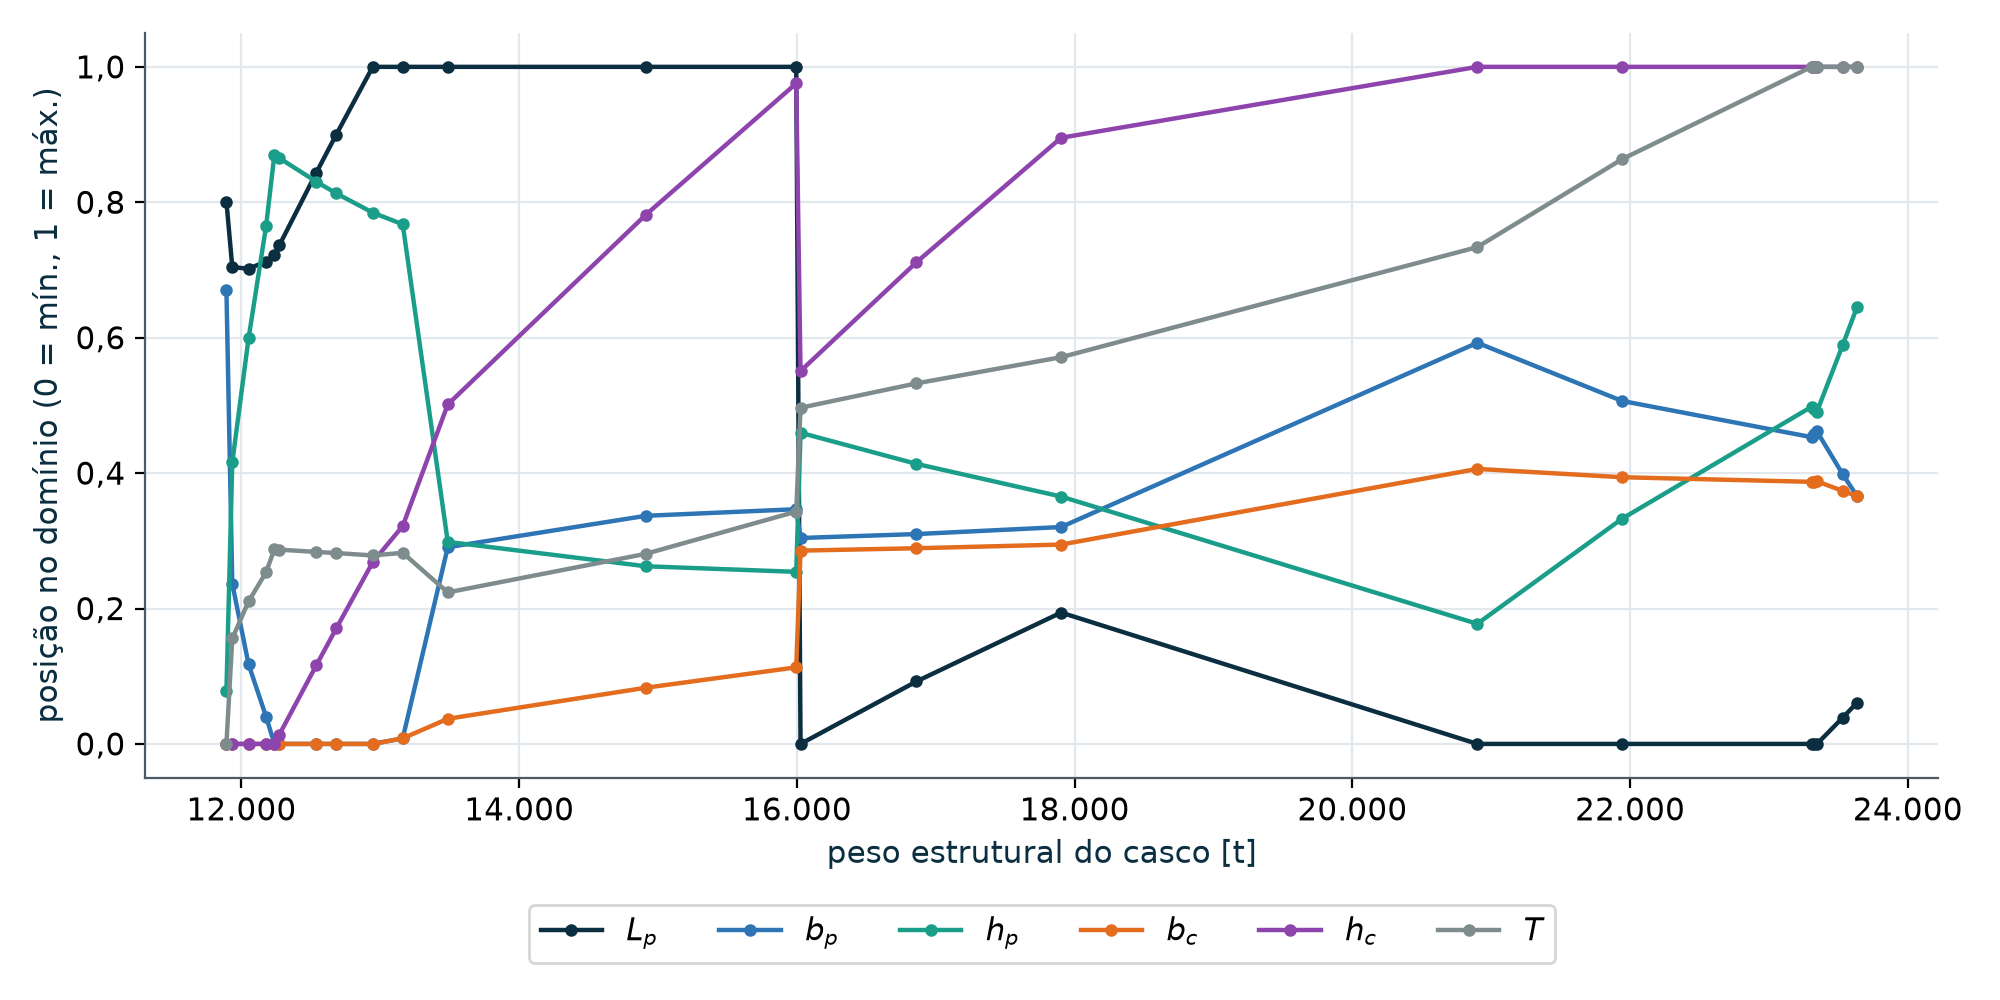
\includegraphics[width=0.88\textwidth]{12_variaveis_fronteira.png}
\caption{Variáveis de projeto normalizadas pelos limites ao longo da fronteira.}\label{fig:variaveis}
\end{figure}

% =============================================================================
\section{Ficha técnica comparativa dos três cenários}\label{sec:cenarios}

{\small
\begin{longtable}{lrrr}
\caption{Ficha técnica comparativa na condição de 10\% de lastro.}\label{tab:ficha}\\
\toprule
 & 1. Mín. peso & 2. Mín. \emph{heave} & 3. Escolhida \\
\midrule
\endfirsthead
\toprule
 & 1. Mín. peso & 2. Mín. \emph{heave} & 3. Escolhida \\
\midrule
\endhead
Origem & $w_1 = 0$ & $w_1 = 1$ & $\varepsilon = 1{,}549$ m \\
\linhas{tabelas/tab_ficha_linhas.tex}
\bottomrule
\end{longtable}}

\begin{figure}[H]
\centering
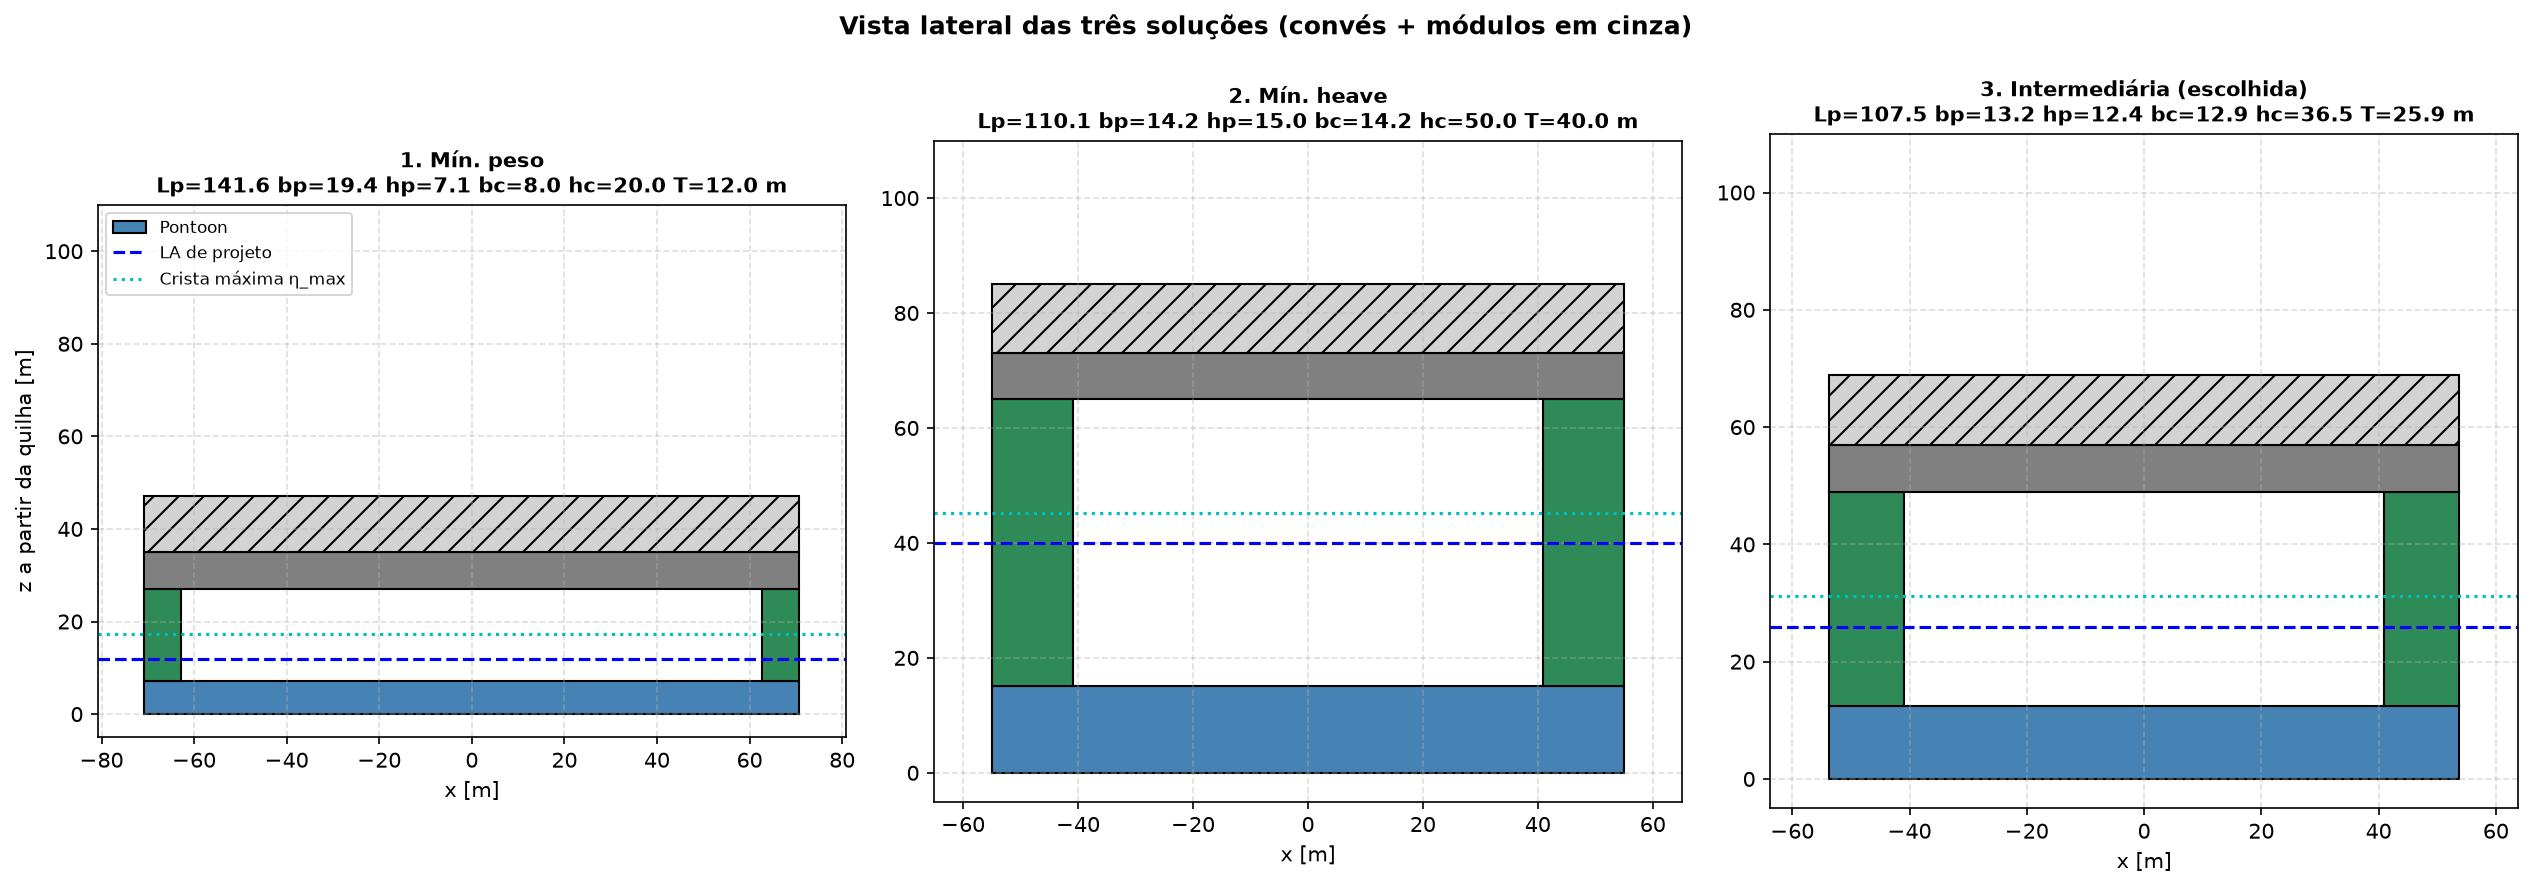
\includegraphics[width=\textwidth]{05_geometria_3_cenarios.png}
\caption{Vista lateral dos três cenários.}\label{fig:geo3}
\end{figure}

\begin{itemize}
\item \textbf{Cenário 1 (mínimo peso, 11.892~t).} Semissubmersível rasa: $b_c$, $h_c$ e $T$ no
limite mínimo, como no caso-base, mas com $L_p = 141{,}6$~m e \emph{pontoons} de 19,4~m de
largura para carregar as 3.991~t de lastro. Tem $T_n = 46{,}5$~s, mas o \emph{heave} é o maior
dos três ($\Hz/H_s = 42\%$) e o ângulo de alagamento é de só 8,7$^\circ$.
\item \textbf{Cenário 2 (mínimo \emph{heave}, 23.634~t).} É o mesmo casco do caso-base: com
$T = 40$~m e $h_c = 50$~m ele já tinha 18.081~t de lastro (37,5\% dos \emph{pontoons}), e a nova
restrição não o afeta.
\item \textbf{Cenário 3 (escolhida, 16.026~t).} Detalhado na Seção~\ref{sec:final}.
\end{itemize}

\begin{figure}[H]
\centering
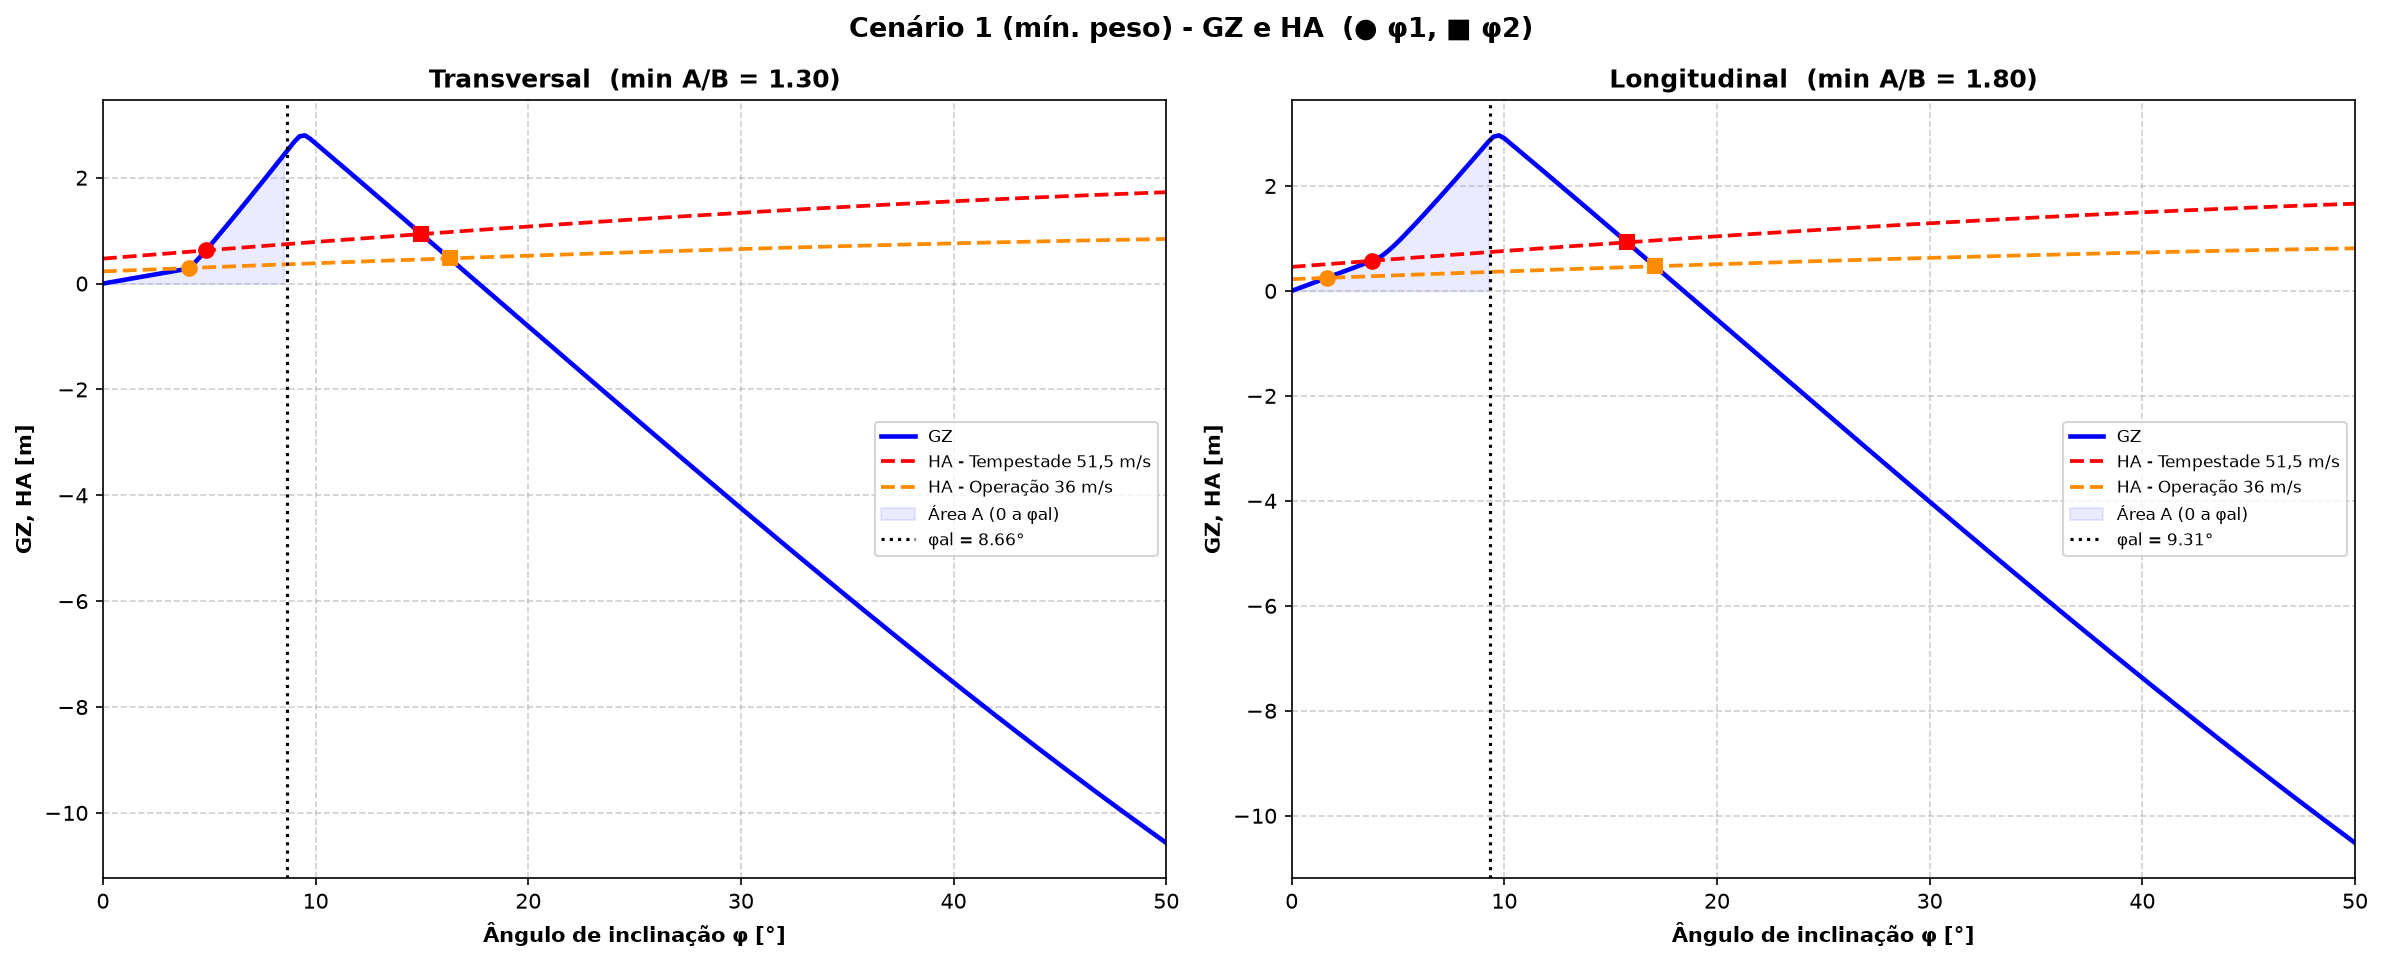
\includegraphics[width=\textwidth]{04a_gz_min_peso.png}
\caption{Cenário 1: curvas GZ e HA.}\label{fig:gz1}
\end{figure}

\begin{figure}[H]
\centering
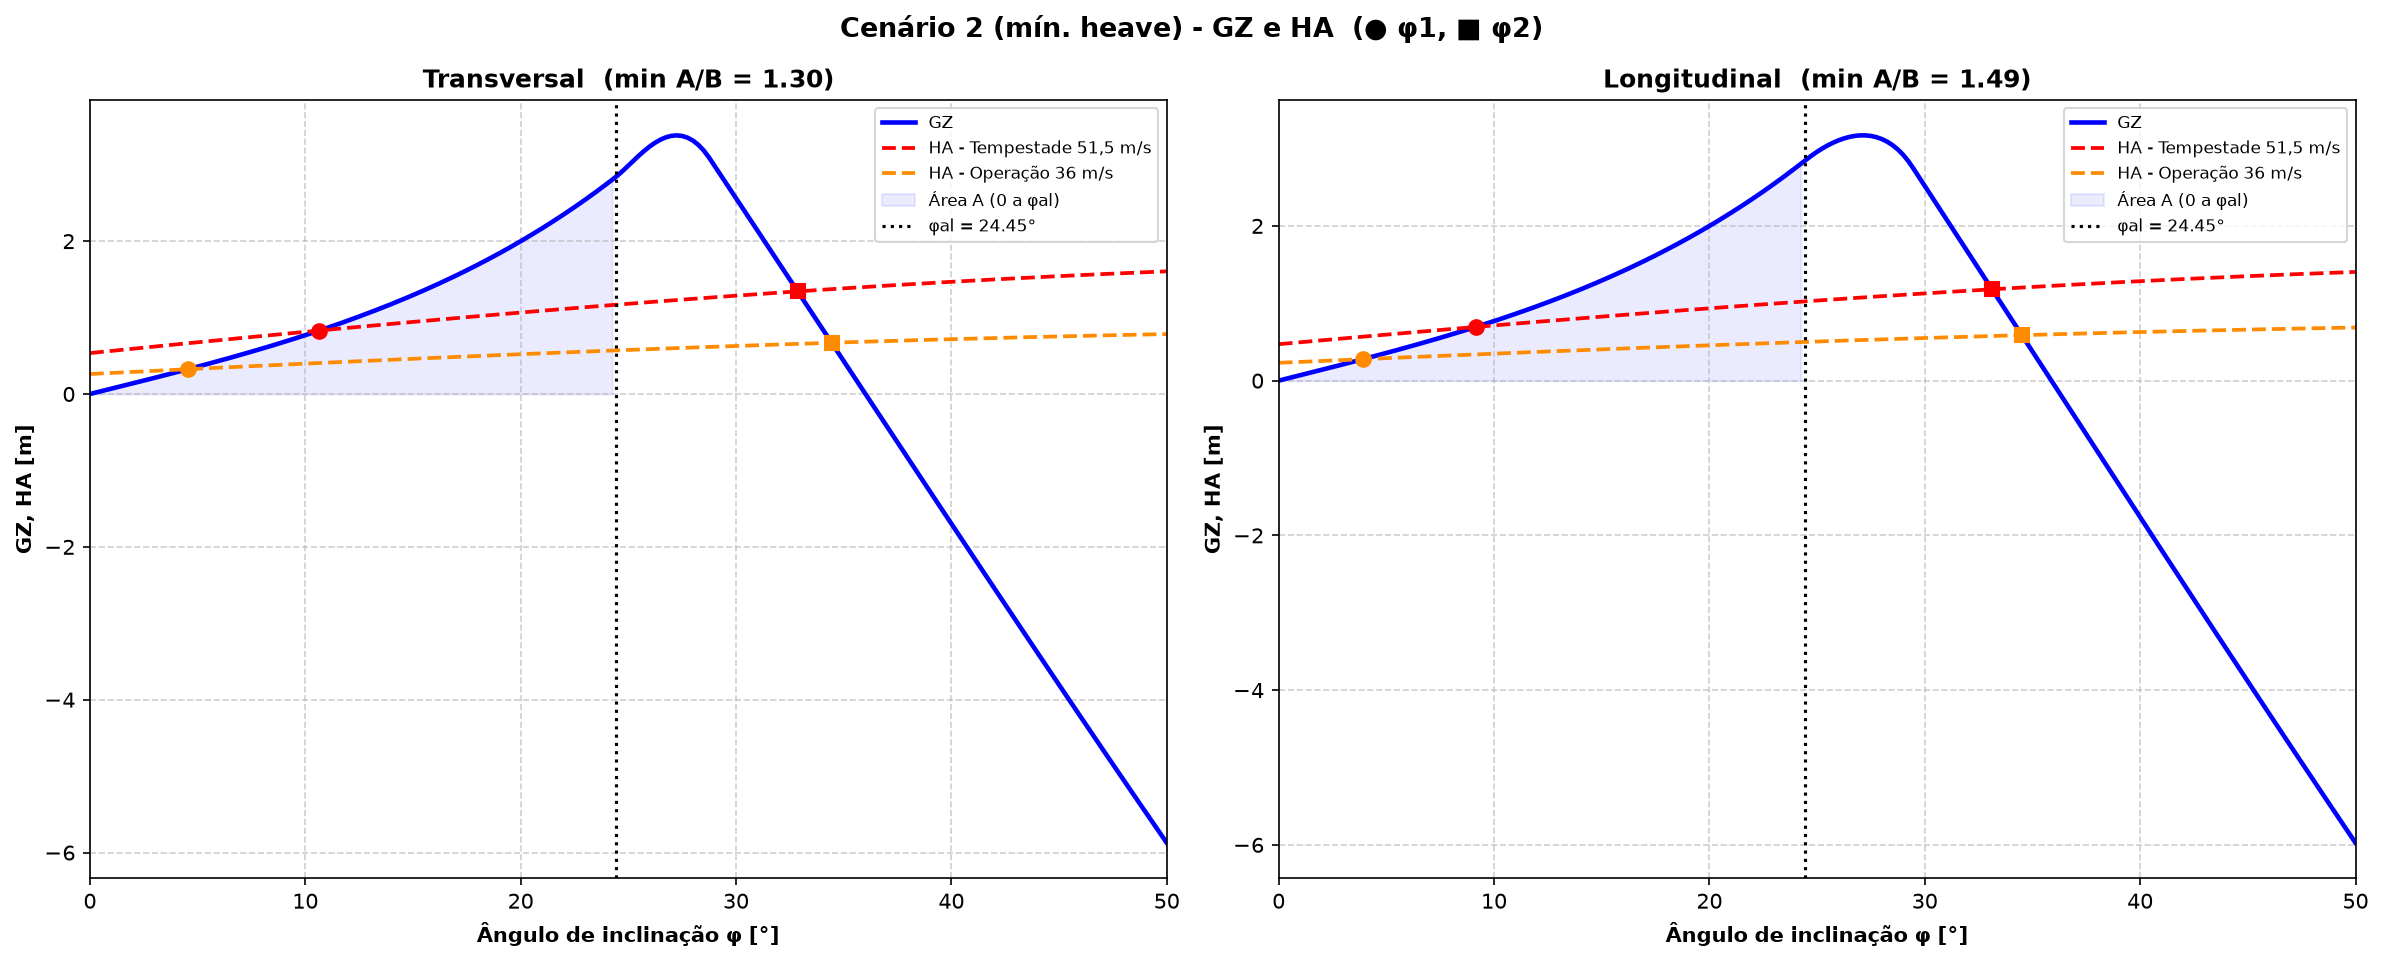
\includegraphics[width=\textwidth]{04b_gz_min_heave.png}
\caption{Cenário 2: curvas GZ e HA.}\label{fig:gz2}
\end{figure}

% =============================================================================
\section{Solução final}\label{sec:final}

\subsection{Dimensões, pesos e centros}

A solução escolhida tem $L_p = 107{,}53$~m (no mínimo dado pela área de convés),
$b_p = 13{,}17$~m, $h_p = 12{,}43$~m, $b_c = 12{,}85$~m, $h_c = 36{,}52$~m e $T = 25{,}90$~m.

\begin{table}[H]
\centering
\caption{Pesos e centros da solução final.}\label{tab:pesos}
\begin{tabular}{lrrr}
\toprule
Item & Peso [t] & VCG [m] & Momento [t$\cdot$m] \\
\midrule
Planta de produção & 13.188,2 & 62,96 & 830.293 \\
Estrutura do convés & 4.615,9 & 52,96 & 244.444 \\
Carga operacional & 4.615,9 & 52,96 & 244.444 \\
\emph{Pontoons} & 9.509,1 & 6,22 & 59.118 \\
Colunas & 6.516,9 & 30,70 & 200.040 \\
\emph{Risers} & 1.808,9 & 48,96 & 88.559 \\
Amarração & 1.356,7 & 48,96 & 66.419 \\
Lastro (nos pontoons) & 3.611,0 & 0,62 & 2.246 \\
\midrule
\textbf{Total ($=\Delta$)} & \textbf{45.222,6} & \textbf{38,38} & \textbf{1.735.562} \\
\bottomrule
\end{tabular}

\end{table}

As 3.611~t de lastro ocupam 10\% do volume dos \emph{pontoons}, com nível de 1,25~m e centro a
0,62~m da quilha. Com KB = 8,83~m e $KM_T = 42{,}38$~m, resulta $GM_T = 4{,}00$~m e
$GM_L = 4{,}22$~m. O KG de 38,38~m é 4,44~m menor que o do caso-base.

\subsection{Estabilidade e critério de vento}

\begin{figure}[H]
\centering
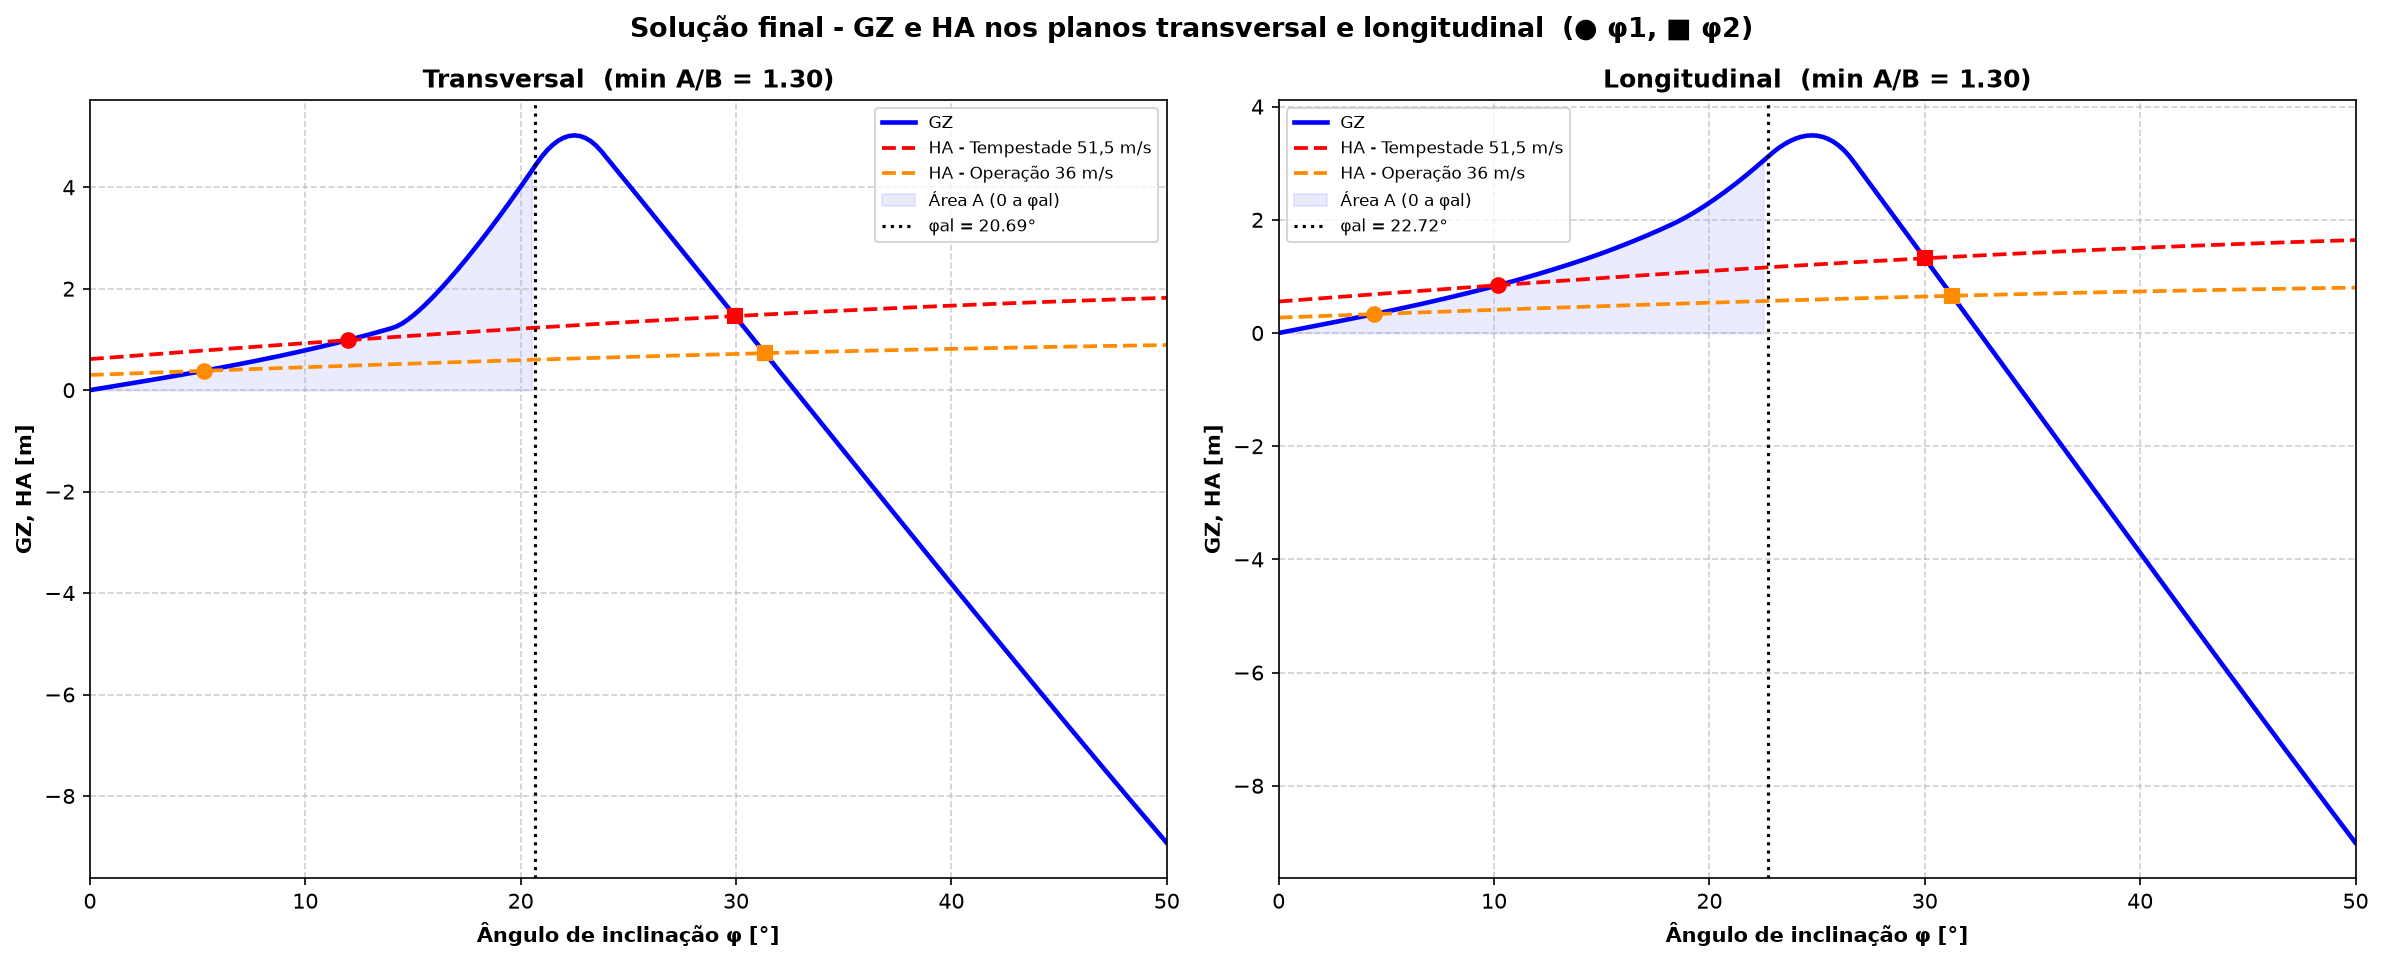
\includegraphics[width=\textwidth]{02_gz_ha_solucao_final.png}
\caption{Solução final: curvas GZ e HA nos dois planos, com $\phial$ indicado
($\bullet$ $\varphi_1$, $\blacksquare$ $\varphi_2$).}\label{fig:gzfinal}
\end{figure}

\begin{table}[H]
\centering
\caption{Forças e braços de vento por parcela na solução final.}\label{tab:ventof}
\small
\begin{tabular}{lrrrrrrrr}
\toprule
 & & & & & \multicolumn{2}{c}{Força [kN]} & \multicolumn{2}{c}{Braço [m]} \\
\cmidrule(lr){6-7}\cmidrule(lr){8-9}
Parcela & Área [m$^2$] & $z$ [m] & $C_s$ & $C_h$ & 51,5 m/s & 36 m/s & Transv. & Long. \\
\midrule
Colunas (4) & 1.185,4 & 11,53 & 1,0 & 1,00 & 1.920,9 & 938,6 & 28,55 & 24,56 \\
\emph{Deck box} & 860,2 & 27,05 & 1,0 & 1,10 & 1.533,5 & 749,3 & 44,08 & 40,08 \\
Módulos & 1.290,4 & 37,05 & 1,1 & 1,20 & 2.760,2 & 1.348,8 & 54,08 & 50,08 \\
Face inferior & 11.562,9 & 23,05 & 1,0 & 1,10 & 20.611,7 & 10.071,7 & 40,08 & 36,08 \\
\bottomrule
\end{tabular}

\end{table}

\begin{table}[H]
\centering
\caption{Momentos de vento por parcela na solução final [kN$\cdot$m].}\label{tab:ventom}
\small
\begin{tabular}{lrrrr}
\toprule
 & \multicolumn{2}{c}{Transversal} & \multicolumn{2}{c}{Longitudinal} \\
\cmidrule(lr){2-3}\cmidrule(lr){4-5}
Parcela & 51,5 m/s & 36 m/s & 51,5 m/s & 36 m/s \\
\midrule
Colunas (4) & 54.839 & 26.797 & 47.172 & 23.050 \\
\emph{Deck box} & 67.589 & 33.027 & 61.468 & 30.036 \\
Módulos & 149.262 & 72.936 & 138.245 & 67.552 \\
\midrule
$HM_0$ & 271.690 & 132.759 & 246.886 & 120.639 \\
$HM_{ud}$ (face inferior) & 826.039 & 403.637 & 743.769 & 363.437 \\
\bottomrule
\end{tabular}

\end{table}

\begin{table}[H]
\centering
\caption{Critério de áreas da solução final nos quatro casos.}\label{tab:criterio}
\small\setlength{\tabcolsep}{4pt}
\begin{tabular}{llrrrrrrrc}
\toprule
Plano & Vento & $z_{CLR}$ [m] & $HA(0)$ [m] & $\varphi_1$ [$^\circ$] & $\varphi_2$ [$^\circ$] &
$\phial$ [$^\circ$] & $A$ [m$\cdot$rad] & $B$ [m$\cdot$rad] & $A/B$ \\
\midrule
\linhas{tabelas/tab_criterio_linhas.tex}
\bottomrule
\end{tabular}
\end{table}

O critério é atendido nos quatro casos, com o mínimo de 1,303 sob tempestade no plano
transversal; o longitudinal fica em 1,304. Em todos os casos $\varphi_2 > \phial$ e a GZ é
positiva até $\phial$ (20,7$^\circ$ no plano transversal e 22,7$^\circ$ no longitudinal). A face
inferior do convés gera 3,0 vezes o momento $HM_0$ das demais parcelas. Sob tempestade, a
plataforma inclina 12,0$^\circ$ em equilíbrio no plano transversal, contra 14,1$^\circ$ no
caso-base.

\subsection{\emph{Heave}}

\begin{figure}[H]
\centering
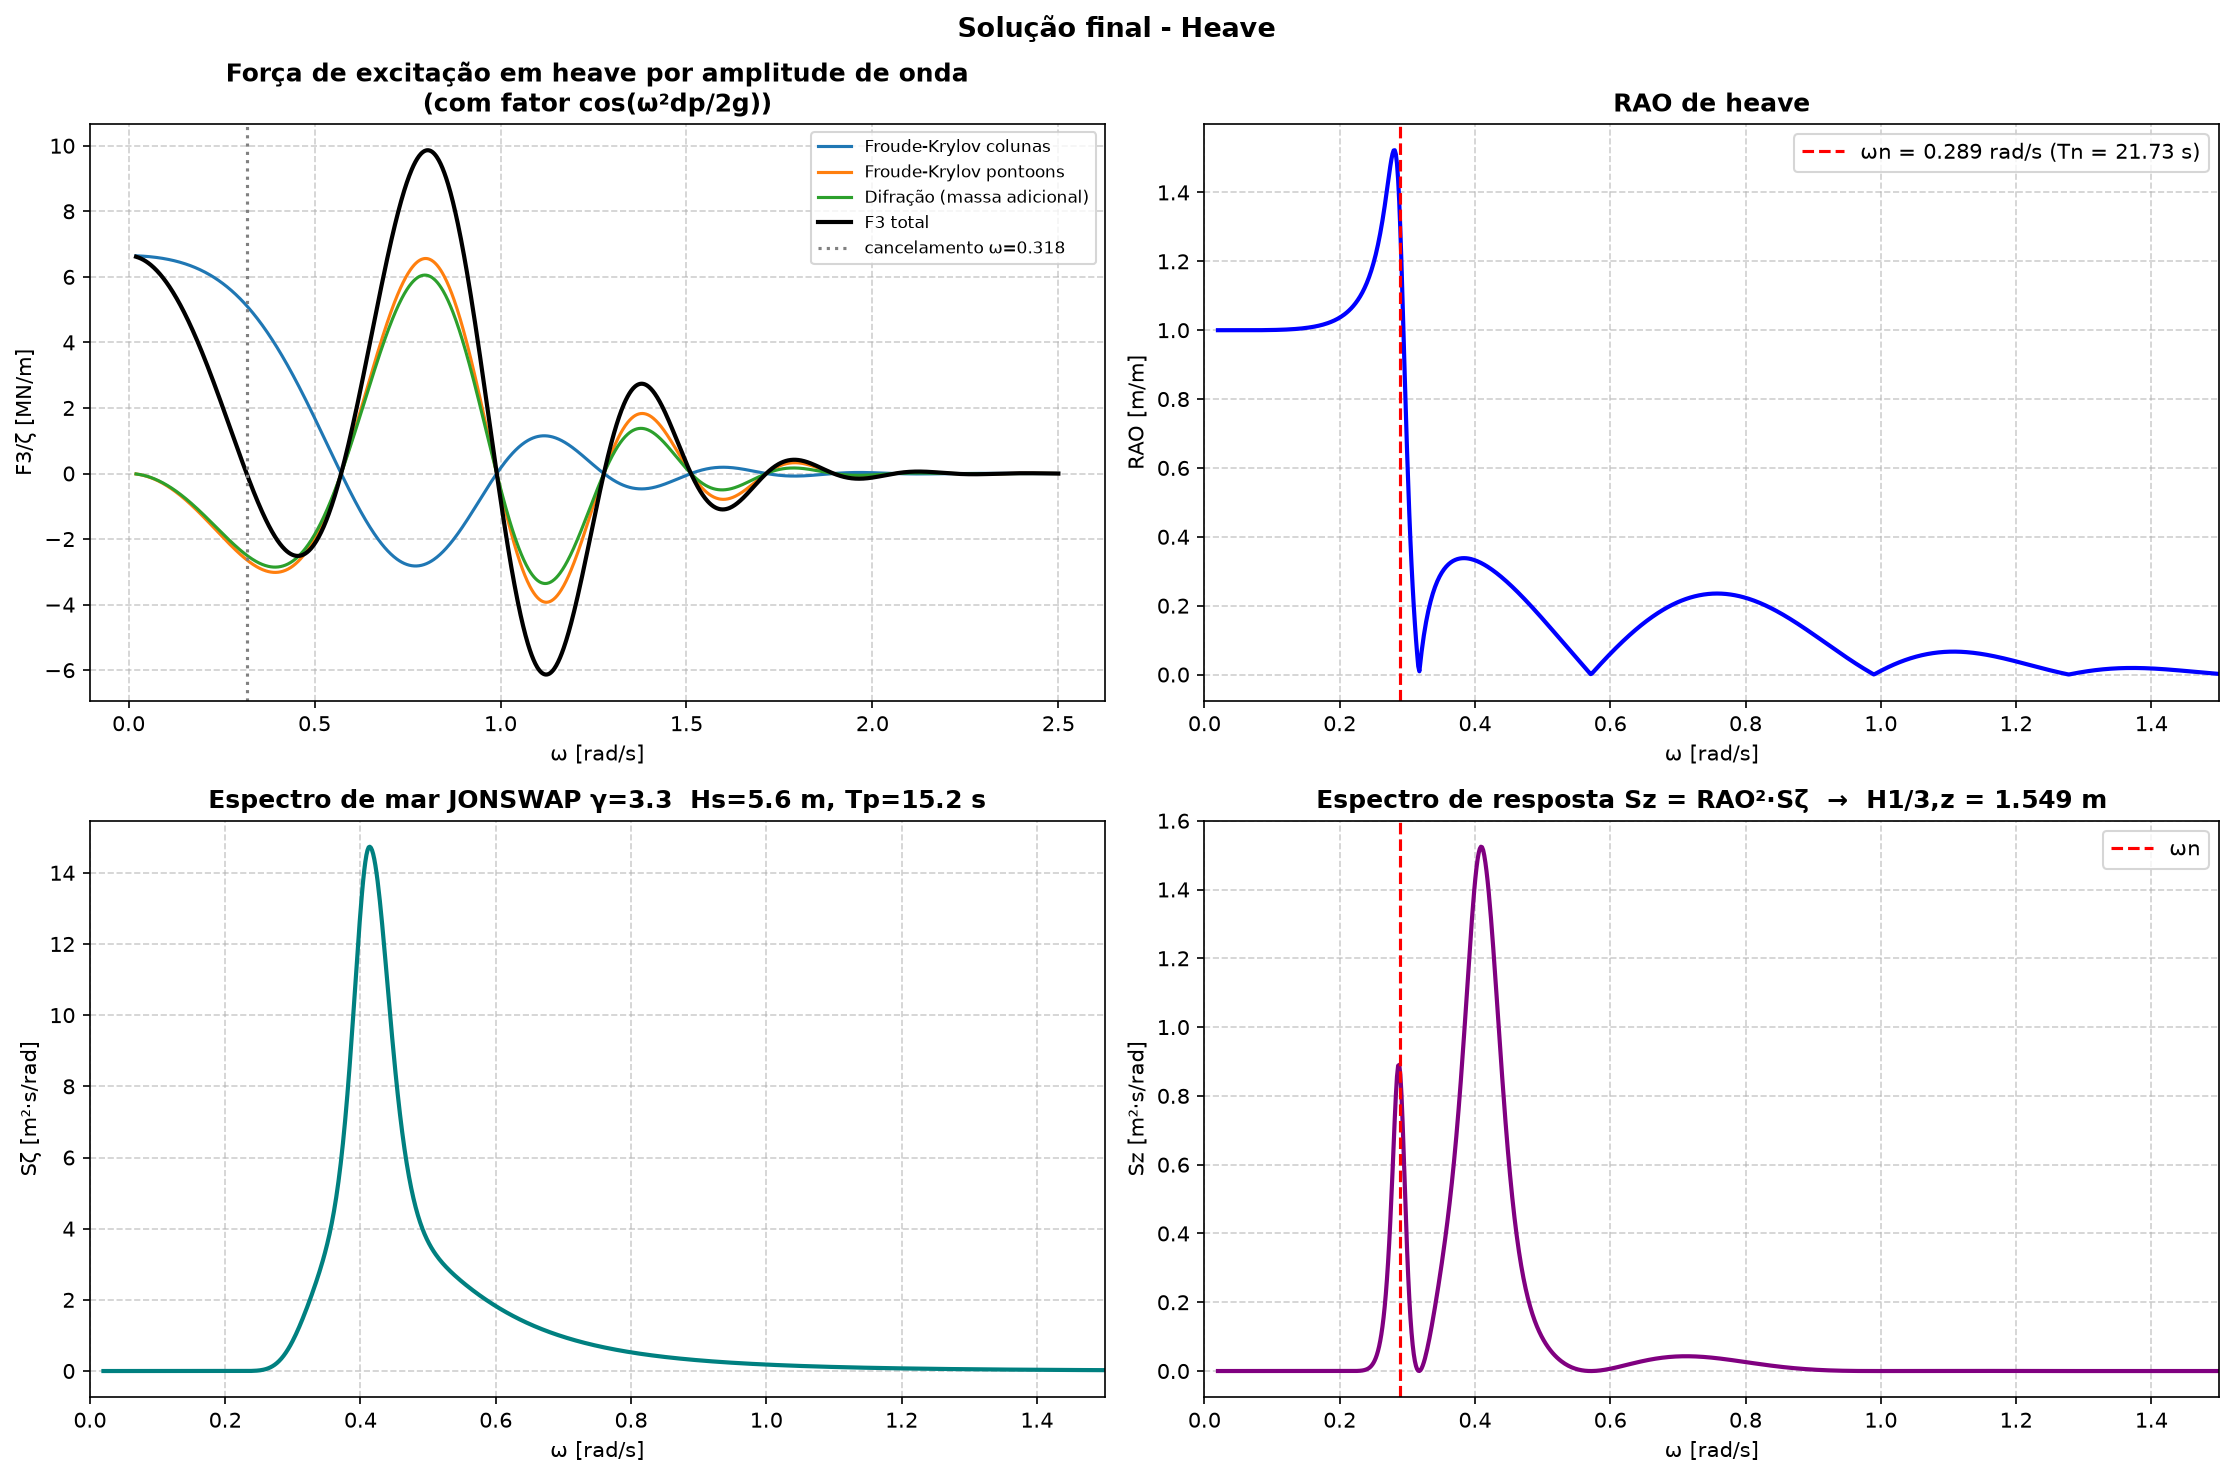
\includegraphics[width=\textwidth]{03_heave_solucao_final.png}
\caption{Solução final: força de excitação, RAO, espectro do mar e espectro de resposta.}\label{fig:heave}
\end{figure}

\begin{table}[H]
\centering
\caption{Resultados de \emph{heave} da solução final.}\label{tab:heave}
\begin{tabular}{lr@{\hspace{1.5cm}}lr}
\toprule
Grandeza & Valor & Grandeza & Valor \\
\midrule
$\Delta$ [t] & 45.223 & $\omega_n$ [rad/s] & 0,2892 \\
$C_A$ & 1,498 & $T_n$ [s] & 21,73 \\
$l_d$ [m] & 81,82 & $\omega$ de cancelamento [rad/s] & 0,318 \\
$A_{33}$ [t] & 34.223 & RAO máximo & 1,52 \\
$C_{33}$ [kN/m] & 6.645 & RAO no pico do mar & 0,32 \\
$B_{33}$ [kN$\cdot$s/m] & 2.298 & $m_{0z}$ [m$^2$] & 0,1500 \\
 & & $\Hz$ ($\gamma = 3{,}3$ / $\gamma = 1$) [m] & 1,549 / 1,456 \\
\bottomrule
\end{tabular}

\end{table}

O período natural de 21,73~s fica 8,6\% acima do limite de 20~s. A força de excitação se anula
em 0,318~rad/s, logo acima de $\omega_n = 0{,}289$~rad/s, o que limita o pico do RAO a 1,52. No
pico do mar ($\omega_p = 0{,}413$~rad/s) o fator de defasagem vale 0,680 e o RAO é 0,32; o
espectro de resposta tem um pico pequeno em $\omega_n$ e o principal no pico da onda. O
$\Hz = 1{,}549$~m (28\% de $H_s$) é praticamente o do caso-base.

\subsection{\emph{Air gap}}

\begin{table}[H]
\centering
\caption{Verificação do \emph{air gap} da solução final.}\label{tab:airgap}
\begin{tabular}{lr}
\toprule
Grandeza & Valor [m] \\
\midrule
$\eta_{max} = 1{,}86 \times 5{,}6/2$ & 5,208 \\
$z_{min} = -1{,}86 \times 1,549/2$ & $-1,441$ \\
$a_{\text{mín}} = \eta_{max} - z_{min}$ & 6,649 \\
$a = h_p + h_c - T$ & 23,055 \\
Folga $a - a_{\text{mín}}$ & 16,406 \\
\bottomrule
\end{tabular}

\end{table}

A folga de 16,4~m continua ampla: a altura das colunas é definida pelo ângulo de alagamento do
critério de vento, e não pela crista da onda.

\subsection{Tabela-resumo das restrições}

\begin{table}[H]
\centering
\caption{Valor de cada restrição na solução final e folga em relação ao limite.}\label{tab:resumo}
\small
\begin{tabular}{llrcrrrl}
\toprule
Restrição & Unid. & Valor & & Limite & Folga & Folga [\%] & \\
\midrule
\linhas{tabelas/tab_restricoes_linhas.tex}
\bottomrule
\end{tabular}
\end{table}

Ficam ativas a área de convés ($L_p$ no mínimo), o $GM_T$ máximo, o lastro mínimo de 10\% e o
critério de áreas.

\subsection{Justificativa da escolha}

A solução 3 é o ponto da fronteira mais próximo do ponto utópico no plano normalizado. Em
relação ao cenário 1, ela aumenta o peso do casco em 34,8\% e reduz o $\Hz$ em 34,3\%; em relação
ao cenário 2, economiza 32,2\% do peso com $\Hz$ 48,5\% maior. Entre os extremos, cortar o
\emph{heave} em 56\% custa +99\% de peso; a solução escolhida captura 62\% do ganho de movimento
com 35\% do acréscimo de massa.

\begin{table}[H]
\centering
\caption{Custo marginal de redução do \emph{heave}.}\label{tab:custo}
\begin{tabular}{lrrr}
\toprule
Trecho & Peso adicional & Redução de $\Hz$ & Custo [t/mm] \\
\midrule
\linhas{tabelas/tab_custo_linhas.tex}
\bottomrule
\end{tabular}
\end{table}

Depois da solução escolhida, cada milímetro de \emph{heave} custa 2,9 vezes mais aço. Ela tem
ângulo de alagamento de 20,7$^\circ$, contra 8,7$^\circ$ do cenário de mínimo peso. Diferente do
caso-base, uma variável fica no limite: $L_p$ está no mínimo, mas esse limite é a própria
restrição de área de convés, e não uma escolha arbitrária de domínio.

% =============================================================================
\section{Comparação com o caso-base}\label{sec:comparacao}

\begin{table}[H]
\centering
\caption{Os três cenários no caso-base e na condição de 10\% de lastro.}\label{tab:cenbase}
\begin{tabular}{lrrrr}
\toprule
Cenário & \multicolumn{2}{c}{Peso do casco [t]} & \multicolumn{2}{c}{$\Hz$ [m]} \\
\cmidrule(lr){2-3}\cmidrule(lr){4-5}
 & Caso-base & Lastro $\ge$ 10\% & Caso-base & Lastro $\ge$ 10\% \\
\midrule
1 · Mín. peso & 10.346 & 11.892 & 2,366 & 2,359 \\
2 · Mín. \emph{heave} & 23.634 & 23.634 & 1,043 & 1,043 \\
3 · Escolhida & 14.998 & 16.026 & 1,552 & 1,549 \\
\bottomrule
\end{tabular}

\end{table}

\begin{figure}[H]
\centering
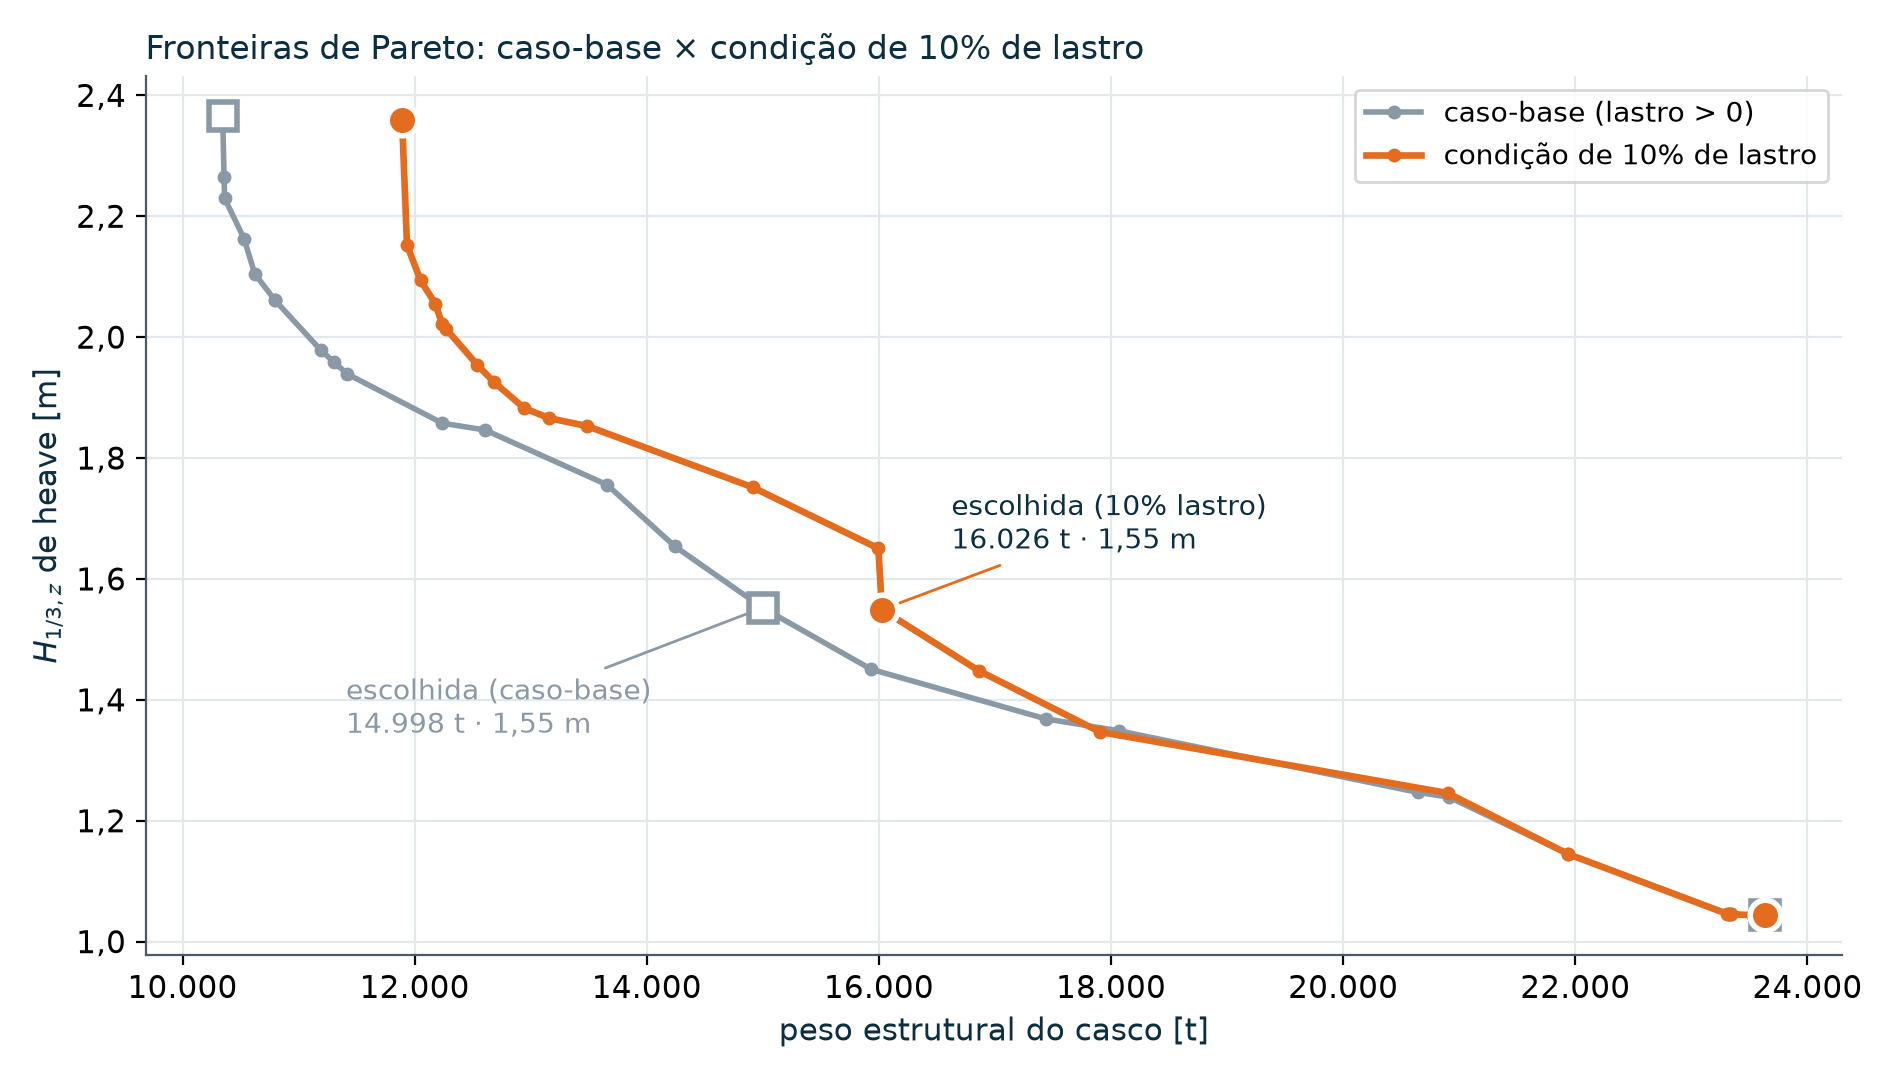
\includegraphics[width=0.85\textwidth]{11_fronteiras_base_x_lastro10.png}
\caption{Fronteiras de Pareto do caso-base e da condição de 10\% de lastro.}\label{fig:fronteiras}
\end{figure}

\begin{table}[H]
\centering
\caption{Solução escolhida: caso-base contra condição de 10\% de lastro.}\label{tab:comparacao}
\begin{tabular}{lrrr}
\toprule
Grandeza & Caso-base & Lastro $\ge$ 10\% & Variação \\
\midrule
\linhas{tabelas/tab_comparacao_linhas.tex}
\bottomrule
\end{tabular}
\end{table}

\begin{itemize}
\item \textbf{Fronteira.} A restrição desloca a parte leve da fronteira para a direita (o mínimo
peso sobe 14,9\%, de 10.346 para 11.892~t) e deixa intacto o extremo de mínimo \emph{heave}, que já
tinha lastro. Perto da solução escolhida, a fronteira fica cerca de 1.000~t à direita da do
caso-base, para o mesmo \emph{heave}.
\item \textbf{Peso e KG.} As 3.611~t de lastro exigem 4.976~t a mais de deslocamento (+12,4\%),
mas o casco cresce só 1.028~t (+6,9\%): o volume extra vem de \emph{pontoons} mais altos ($h_p$
+2,2~m) e de um calado 1,9~m maior. A água no fundo baixa o KG em 4,44~m.
\item \textbf{Estabilidade.} Com KG mais baixo, o $GM_T = 4$~m é obtido com BM menor
(33,6 contra 39,1~m), e a GZ cresce mais em ângulos grandes. A área $A$ do critério sai com
colunas mais curtas ($h_c$ $-$3,1~m) e $L_p$ no mínimo; $GM_T$ e $A/B$ continuam ativos.
\item \textbf{Hidrodinâmica e \emph{air gap}.} $\Hz$ (1,549 contra 1,552~m) e $T_n$ (21,73
contra 21,85~s) praticamente não mudam; a folga de \emph{air gap} cai 2,8~m, para 16,4~m.
\end{itemize}

% =============================================================================
\section{Comparação com plataformas reais}\label{sec:reais}

O pôster \emph{2011 Worldwide Survey of Semi-FPSs and FPUs}~\cite{poster}, referência [6] do
enunciado, traz as dimensões e o deslocamento de semissubmersíveis de produção reais
(Tabela~\ref{tab:poster} e Figura~\ref{fig:poster}).

\begin{table}[H]
\centering
\caption{Solução escolhida (10\% de lastro) contra as semissubmersíveis do pôster de 2011
($n$ = número de unidades com o dado).}\label{tab:poster}
\small
\begin{tabular}{lrrrrr}
\toprule
Grandeza & $n$ & Mínimo & Mediana & Máximo & G02 (10\%) \\
\midrule
\linhas{tabelas/tab_poster_linhas.tex}
\bottomrule
\end{tabular}
\end{table}

\begin{figure}[H]
\centering
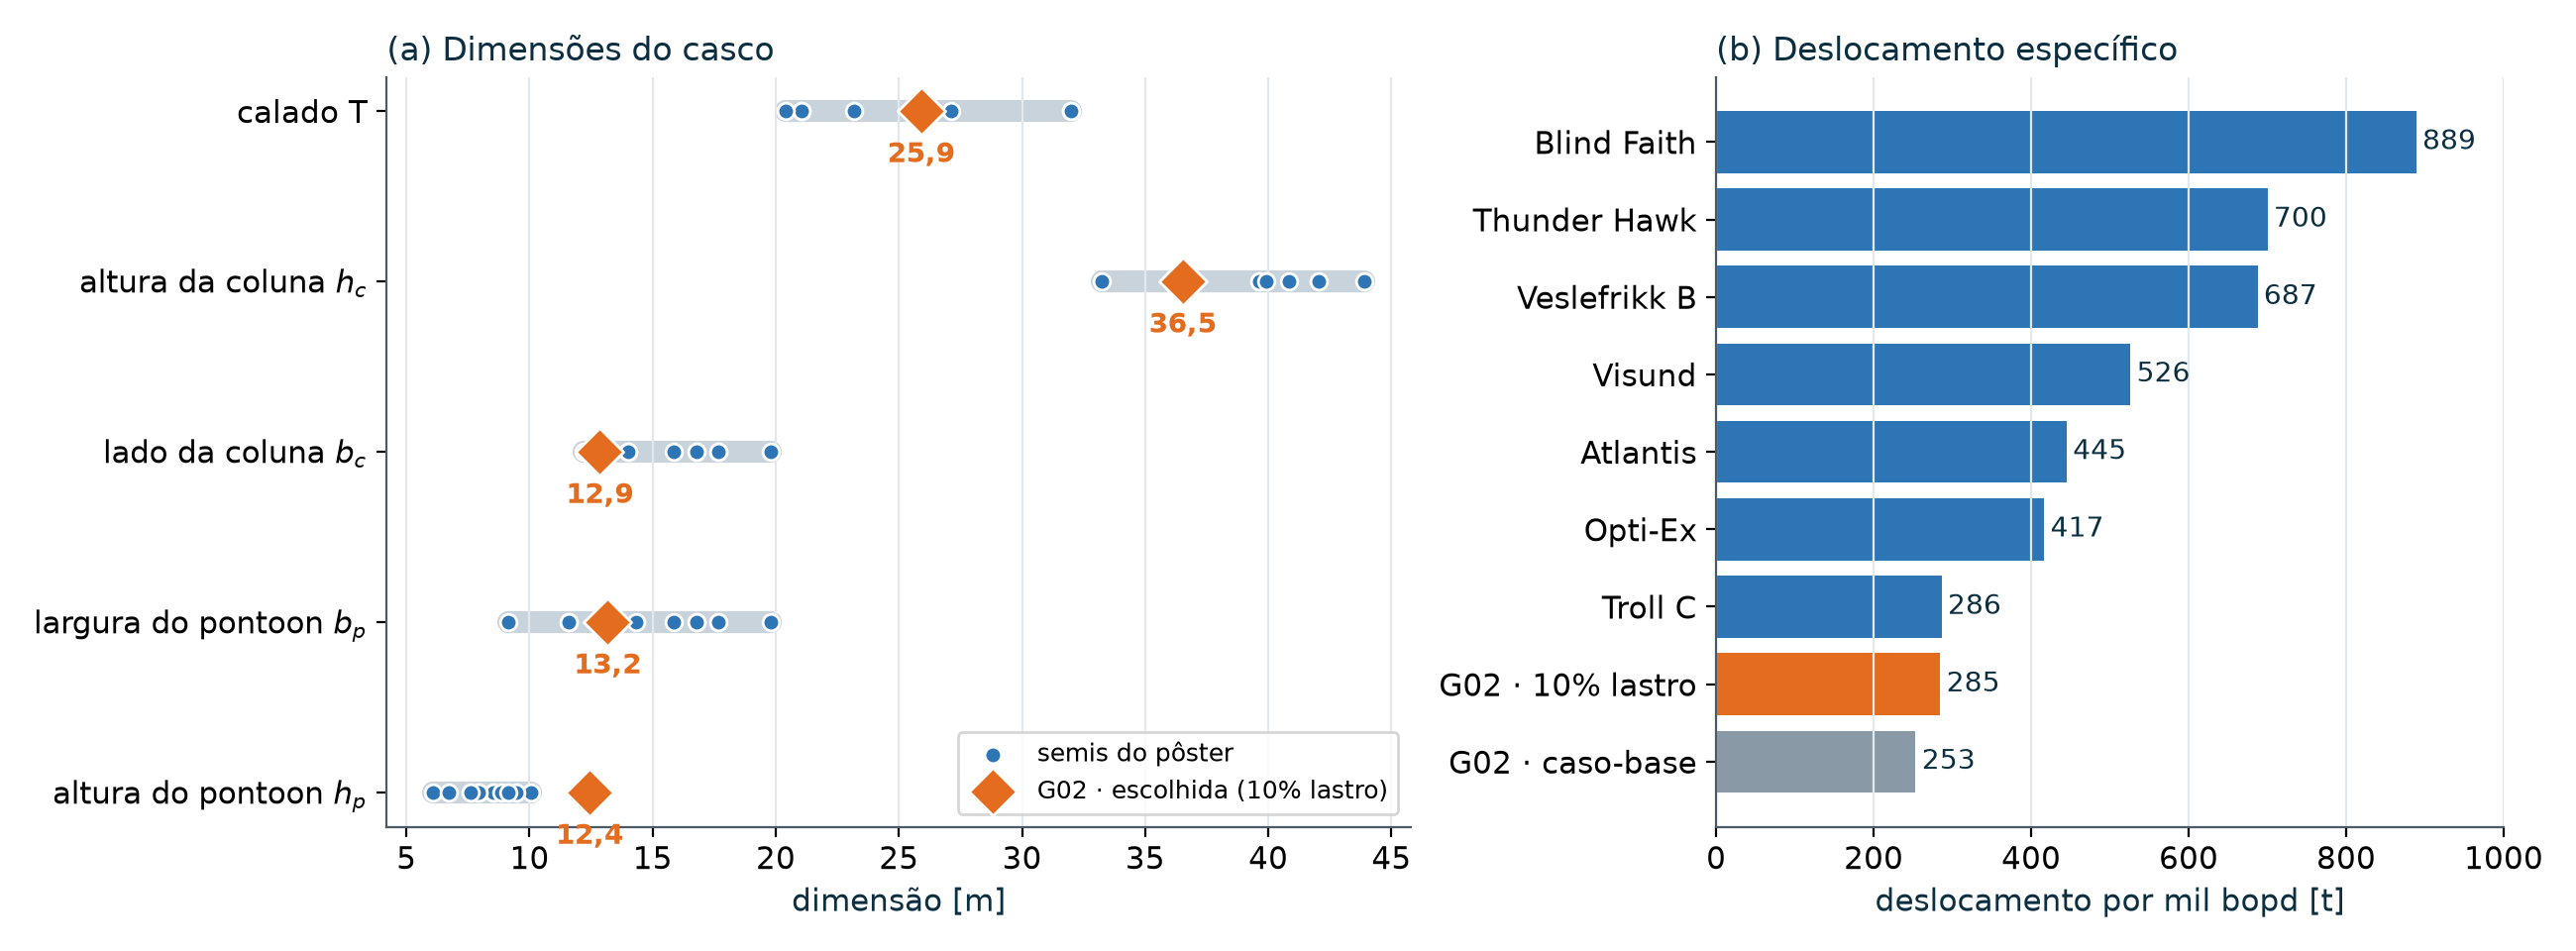
\includegraphics[width=\textwidth]{13_poster2011.png}
\caption{Solução escolhida contra o pôster de 2011: (a) dimensões do casco; (b) deslocamento
por mil bopd.}\label{fig:poster}
\end{figure}

\begin{itemize}
\item \textbf{Deslocamento.} A solução desloca 285~t por mil bopd, o nível da Troll C (286~t), a
unidade mais enxuta do pôster. No caso-base, sem lastro, o valor era 253~t, abaixo de toda a
frota; a diferença confirma que a leveza do caso-base vinha da falta de lastro.
\item \textbf{Dimensões.} Calado, altura e lado da coluna e largura do \emph{pontoon} ficam dentro
da faixa da frota. O \emph{pontoon} (12,4~m) é mais alto que o maior do pôster (10,1~m), efeito
do volume extra necessário para o lastro.
\item \textbf{\emph{Topside}.} O \emph{topside} por mil bopd (141~t) é o mesmo do caso-base e
coincide com a mediana do pôster (145~t).
\item \textbf{Região.} Os análogos reais do Baixo Congo, o FPSO do CLOV~\cite{clov} (160 mil bpd
em 1.291~m) e a Moho/Bilondo, têm casco de navio e armazenam o óleo; uma semissubmersível
exigiria FSO ou oleoduto de 190~km, custo fora do escopo deste modelo.
\end{itemize}

% =============================================================================
\section{Conclusões}

\begin{enumerate}
\item Com lastro mínimo obrigatório de 10\% do volume dos \emph{pontoons}, a fronteira de Pareto
tem 23 pontos, de 11.892~t ($\Hz = 2{,}36$~m) a 23.634~t ($\Hz = 1{,}04$~m), e só 1,0\% do
domínio é viável.
\item O projeto continua governado pela estabilidade: $GM_T = 4$~m e $A/B = 1{,}30$ estão ativos
em toda a fronteira, e a restrição de lastro está ativa em 16 dos 23 pontos.
\item A solução escolhida tem casco de 16.026~t, 3.611~t de lastro, $\Hz = 1{,}55$~m,
$T_n = 21{,}7$~s e $A/B = 1{,}303$; depois dela, reduzir o \emph{heave} custa 2,9 vezes mais aço.
\item Em relação ao caso-base, o lastro custa +6,9\% de casco, reduz o KG em 4,44~m e mantém o
\emph{heave} e o período natural; as duas configurações são tecnicamente válidas e equivalentes
em hidrodinâmica.
\item O deslocamento específico (285~t por mil bopd) passa ao nível da Troll C, a
semissubmersível mais enxuta do pôster de 2011, o que alinha o casco à frota real.
\end{enumerate}

\paragraph{Recomendações.} Adotar esta condição na fase seguinte do projeto; confirmar com o
professor se o gás entra no BOE (+25\% no casco no caso-base); fundamentar $h_m$; incluir roll,
pitch e efeitos não lineares no \emph{air gap} (DNVGL-OTG-13).

% =============================================================================
\begin{thebibliography}{9}
\bibitem{poster} Supan, C. (Mustang Engineering). \emph{2011 Worldwide Survey of Semi-FPSs and
FPUs}. Offshore Magazine, Poster 89, jan. 2011.
\bibitem{c301} DNV. \emph{DNV-OS-C301 -- Stability and Watertight Integrity}, 2013.
\bibitem{modu} IMO. \emph{Code for the Construction and Equipment of Mobile Offshore Drilling
Units (2009 MODU Code)}, Res. A.1023(26), 2009.
\bibitem{c205} DNV. \emph{DNV-RP-C205 -- Environmental Conditions and Environmental Loads}, 2010.
\bibitem{otg13} DNV GL. \emph{DNVGL-OTG-13 -- Prediction of Air Gap for Column-Stabilised
Units}, 2019.
\bibitem{clov} Offshore Technology. \emph{CLOV Development Project, Block 17, Offshore Angola}.
\url{https://www.offshore-technology.com/projects/clov-development-project-angola/}.
\end{thebibliography}

% =============================================================================
\appendix
\section{Fronteira de Pareto completa}\label{ap:fronteira}

\begin{longtable}{rrrrrrrrl}
\caption{Pontos não dominados na condição de 10\% de lastro, ordenados por peso.
SP = soma ponderada; $\varepsilon$ = $\varepsilon$-restrito.}\label{tab:fronteira}\\
\toprule
\# & $L_p$ & $b_p$ & $h_p$ & $b_c$ & $h_c$ & $T$ & $W_{casco}$ [t] & $\Hz$ [m] / origem \\
\midrule
\endfirsthead
\toprule
\# & $L_p$ & $b_p$ & $h_p$ & $b_c$ & $h_c$ & $T$ & $W_{casco}$ [t] & $\Hz$ [m] / origem \\
\midrule
\endhead
\linhas{tabelas/tab_fronteira_linhas.tex}
\bottomrule
\end{longtable}

\section{Reprodução dos resultados}

Na pasta \texttt{condicao\_10pct\_lastro/} do repositório:
\begin{verbatim}
pip install -r ../requirements.txt
python codigo/pnv3425_grupo02_condicao_10pct_lastro.py   # ~3 min em 8 núcleos
python codigo/analises_condicao_10pct_lastro.py           # figuras e tabelas
\end{verbatim}
O primeiro script grava os resultados em \texttt{resultados\_lastro10/}. O segundo usa também
os resultados do caso-base, na pasta \texttt{caso\_base/resultados/}, e gera as tabelas deste
relatório em \texttt{relatorio/tabelas/}. O lastro mínimo pode ser alterado pela variável de ambiente
\texttt{LASTRO\_MIN\_FRAC}.

\end{document}
